\documentclass[12pt]{article}
\usepackage{graphicx} % Required for inserting images
\usepackage{float}
\usepackage{xcolor}
\usepackage{listings}
\usepackage{amsmath}
\usepackage{tabularx}



\usepackage[utf8]{inputenc}
\usepackage[T1]{fontenc}
\usepackage[margin=2.5cm]{geometry}
\usepackage{setspace}
\singlespacing
\usepackage{helvet}
\renewcommand{\familydefault}{\sfdefault}
\usepackage{xcolor}
\usepackage{tcolorbox}
\usepackage{array}
\usepackage{tabularx}
\usepackage{fancyhdr}
\usepackage{hyperref}
\usepackage{parskip}


\title{INF3315 - Privacy Preserving Computation \\ \Large Assignment 3}

\author{Sebastian Mai}
\date{DUE: Monday 2.November.2026}


\begin{document}

\maketitle
\doublespacing

\section{Task 1:}
\textbf{LO1:} explain how linking a de-identified dataset with public data re-identifies people, and measure the risk with k-anonymity and sparse cells.
The medical survey of course contains a lot of sensitive information about diabetes. 
By linking the survey with the pulic information which contains name, pnr, age, zip code etc. using shared attributes such as the age, zip code or county it is possible to associate seemingly 
anonymous medial records with a named individual. Just removing names alone is therefor not sufficient enought to guarantee privacy as other attributes can also work as identifiable attributes allowing us to re-identify people.

In terms of k-anonymity it measures how many individuals share the same combination of identifiers. So generally sepaking the higher the k the better the anonymity.
If $k=1$ then there is only a single person with the same attributes. This means there is a complete and unique re-identification.
In the heatmap all k from 1-4 are marked as sparse cells. A total of 8405 people are uniquely identifiable. 1380 share an attribute and 215 people habe 3 or 4 attributes shared. Noticable is also
that County adds no information that isn't already included in the zip code. For example looking at k=1 the combination of zipcode + age identifies 8405 people uniquely. The combination of zipcode, age and county identifies the same amount.
If zip code is removed it identification becomes much harder as more people are included in a municipality (counties usually have more than a single zipcode)

When looking at what the API reveals about a person, we must say quite a lot. Taking Andrea Antonsen, 21, 0308 then by calling the API with 
getDiabeticsByZip(0308) returns 1, meaning there is only a single person that is diabetic in that county. Then calling getAvgAgeByZip(0308) returns 21. So we also get the age of that person. Checking the pii we can get all other information such as the name.

A little bit more about sparse cells. Looking at the county-age heatmap numbers a total of 3360 contained fewer than 5 people. Those cells contained 52\% all the entire dataset.
Sparse cells pose a privacy risk as fewer people in the combination means also easier indentification. 

\begin{figure}[htbp]
    \centering
    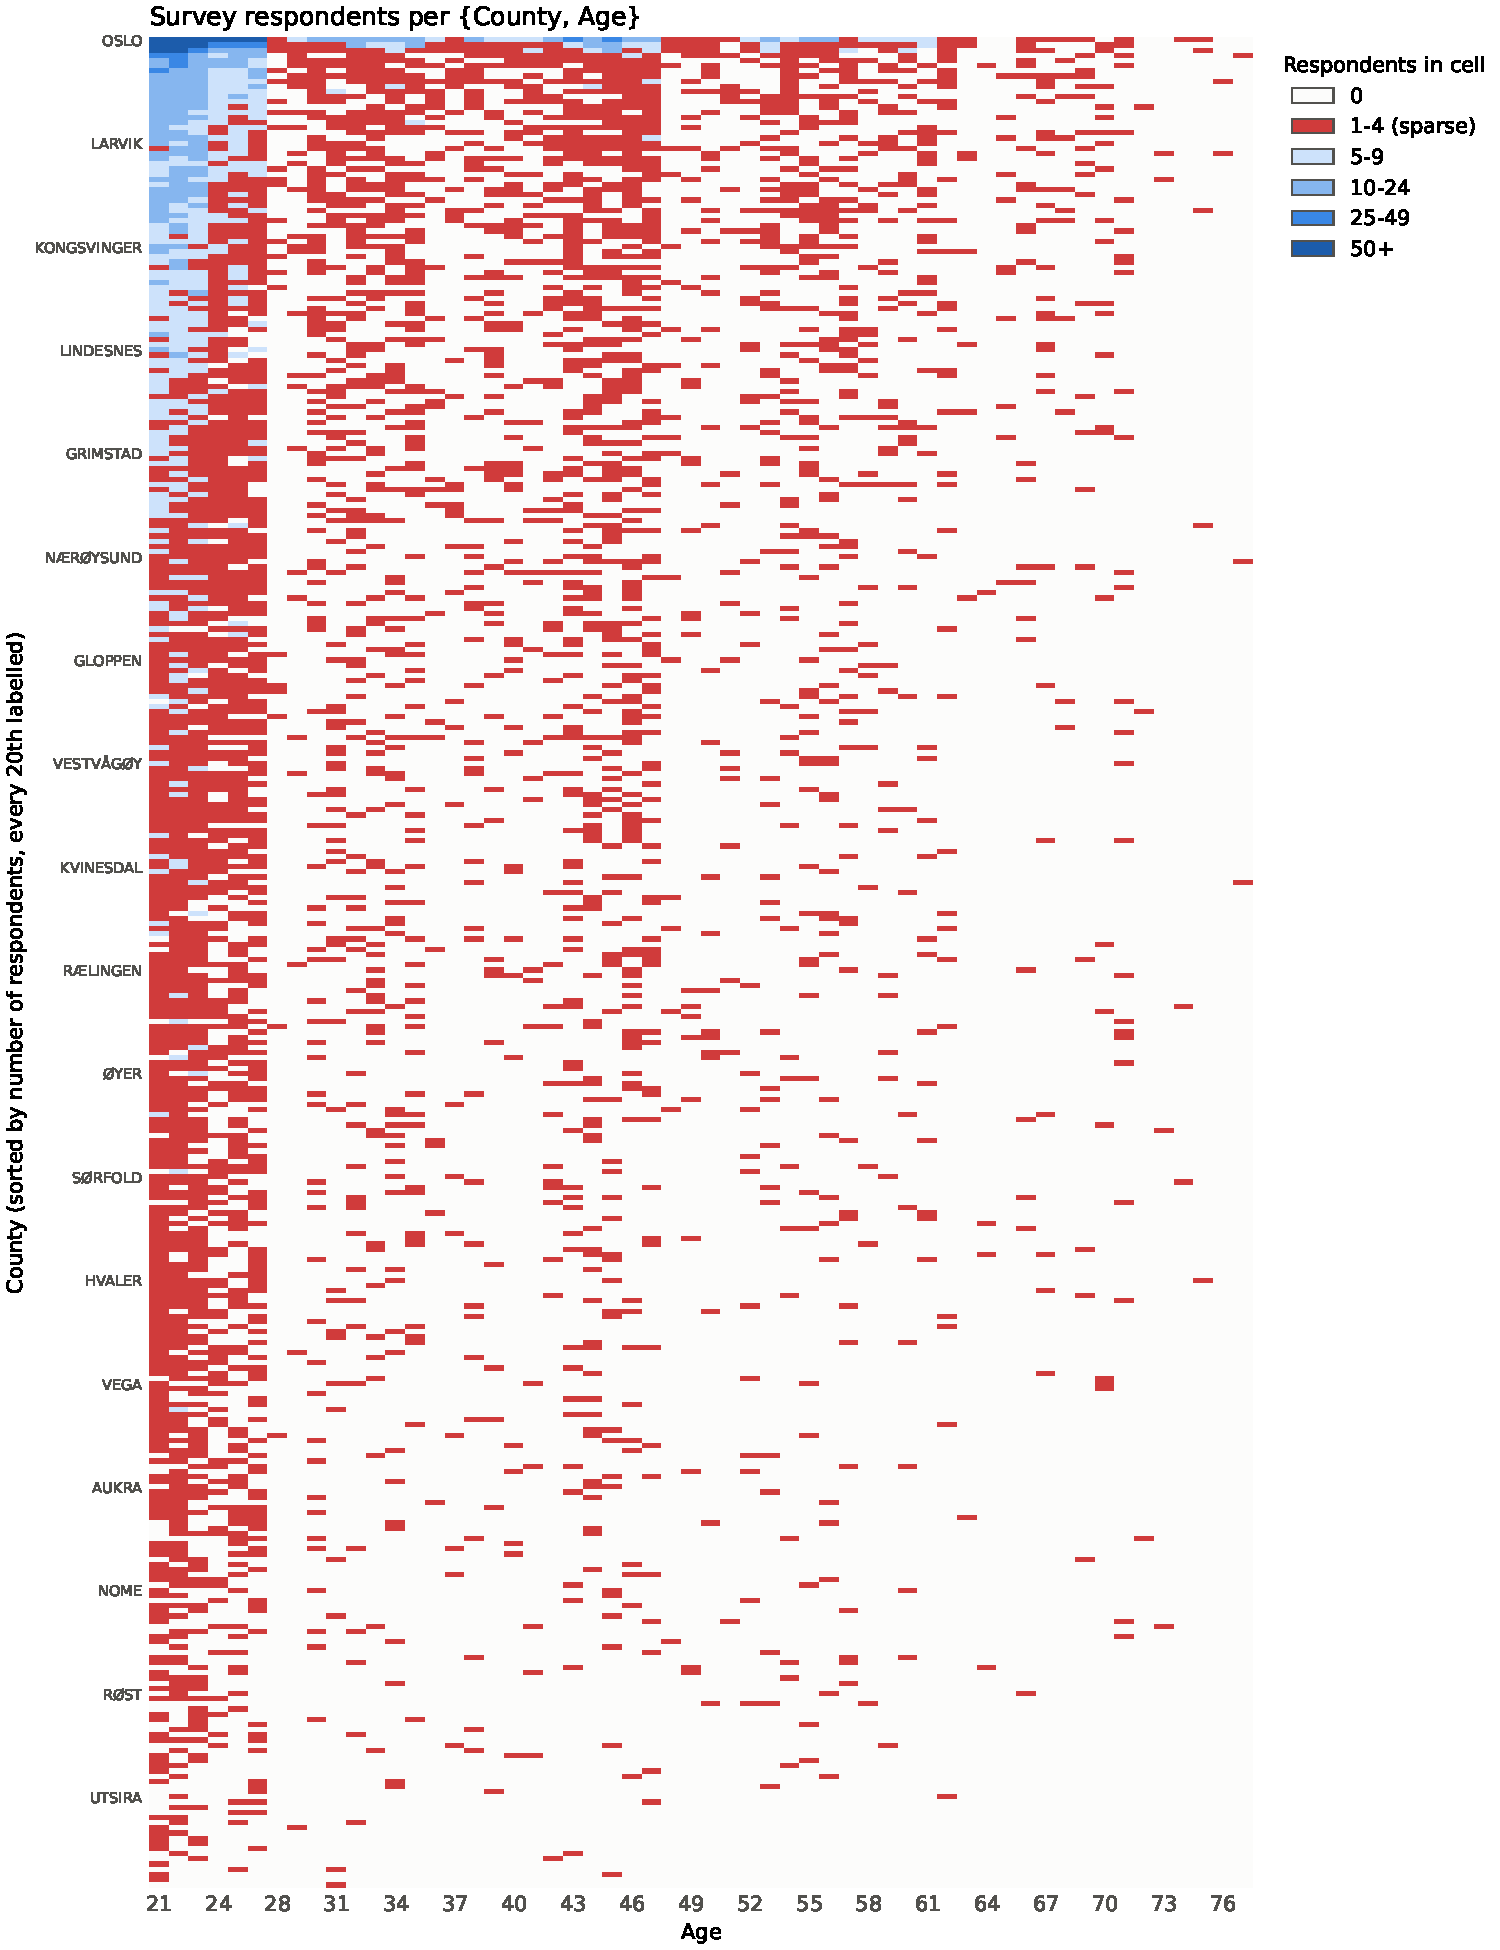
\includegraphics[width=\textwidth,height=0.8\textheight,keepaspectratio]{heatmap_county_age.pdf}
    \caption{Survey respondents per \{County, Age\}. Counties are sorted by number of respondents; cells with 1--4 respondents are marked red as sparse.}
    \label{fig:heatmap}
\end{figure}

\end{document}